%\section{Making It Accurate and Scalable} \label{sec:technicalInno}
\section{Accurate: Selective Inlining}\label{sec:inline}
%In this section, we explain the inlining process, which aims to recover the complete semantics of the binary functions.
\xyx{Inlining is a technique in compilers to optimize the binaries for maximum speed or minimum size~\cite{chang1992profile}.
During compilation, the strategy of inlining is different according to the configured optimization level, which creates the challenge for binary code search. To mitigate this issue, we propose a selective inlining strategy which is based on function invocation patterns. Note that our strategy has a different goal in contrast with compilation process --- ours is for program semantics recovery, while compilers' is for speed or size optimization.}

\subsection{Function Invocation Patterns}
\begin{figure*}[t]
   \centering
   %height=5cm,width=0.8\textwidth
  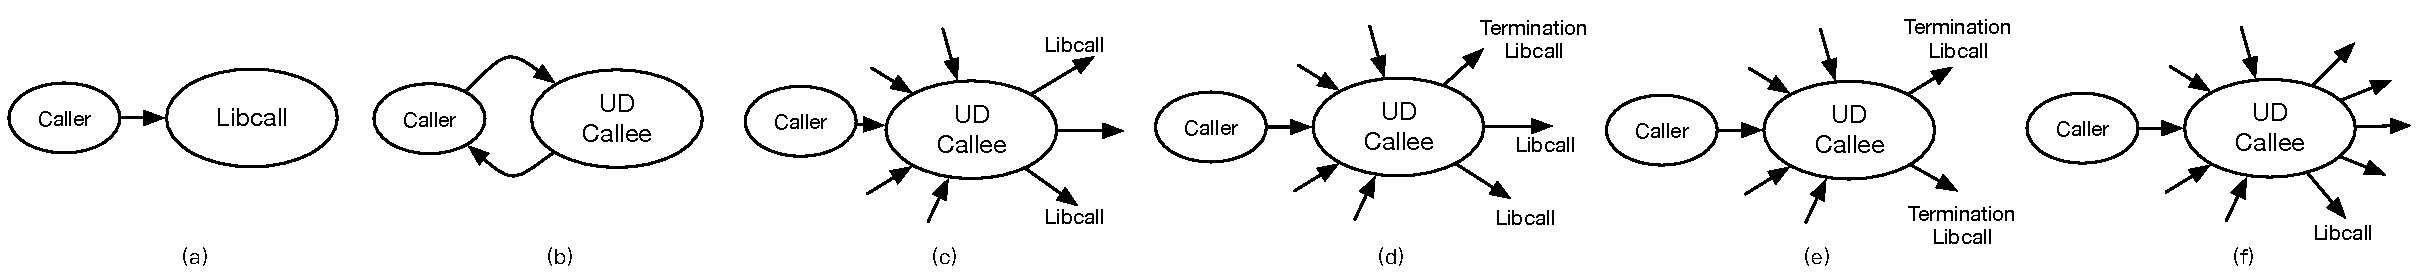
\includegraphics[width=\textwidth]{srj-figures/srj-caller-callee6.pdf}
  %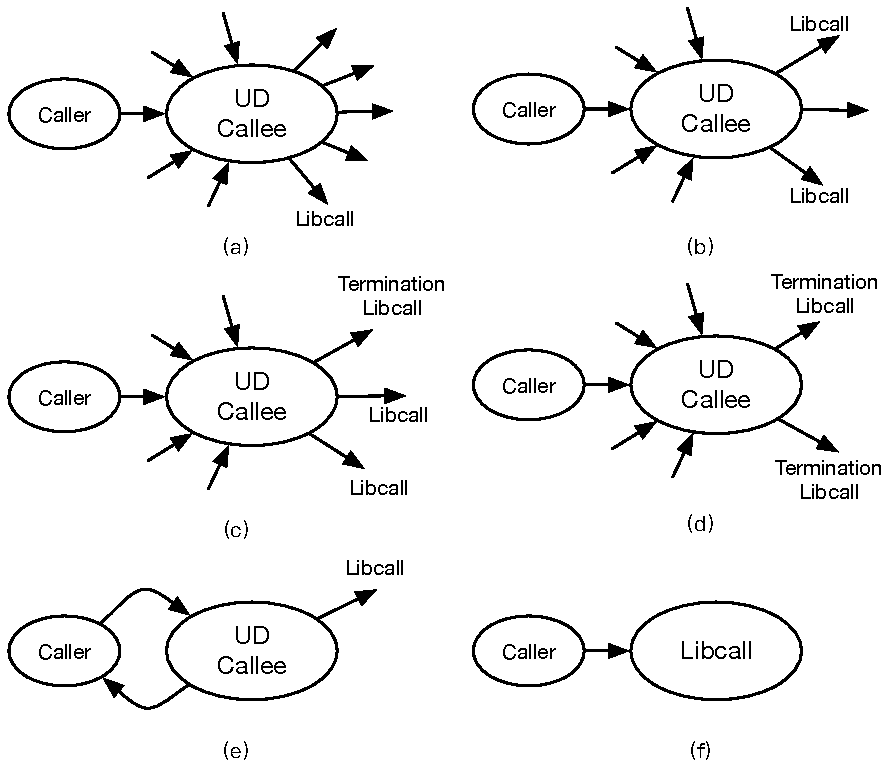
\includegraphics[width=0.45\textwidth]{srj-figures/srj-caller-callee4.pdf}
  \caption{Commonly observed function invocation patterns, where `UD' denotes user-defined callee function. Here, all the incoming and outgoing edges (or calls) represent user-defined functions, unless specified as \textit{Libcall} or \textit{Termination Libcall} next to them} \label{fig:caller-callee} \vspace{-1mm}
\end{figure*}
In order to inline relevant functions, we use the function invocation patterns to guide the inlining decision. Based on our study, six commonly-observed invocation patterns are identified and summarised in Fig.~\ref{fig:caller-callee}.
Incoming (outgoing) edges in Fig.~\ref{fig:caller-callee} represent the incoming (outgoing) calls to (from) the function.
%Four out of six patterns refer to the functions to be inlined, while the other two are not.
Here, we elaborate the six patterns as follows.

\noindent\textbf{Case 1:} Fig.~\ref{fig:caller-callee}(a) depicts the direct invocation of standard C library function(s) by the caller function under investigation. To recover the semantics, it is essential to understand the semantics of called library function(s). Hence, the library function is inlined into the caller function.  Currently, we only consider the most common standard C library functions --- in total 60 functions,
%(e.g., \texttt{memcpy} and \texttt{strlen})
from both Linux (\texttt{libc}) and Windows (\texttt{msvcrt}), for inlining. This list can be further extended when necessary.

\noindent\textbf{Case 2:} Fig.~\ref{fig:caller-callee}(b) depicts the case of a recursive relationship between the caller and the UD (user-defined) callee function $f$. Hence, we inline $f$ into its caller. Note that the recursive functions are, unlike in compilers, inlined only once. For example, \texttt{gcc} has a default inlining depth of 8 for recursive functions.

\noindent\textbf{Case 3:} Fig.~\ref{fig:caller-callee}(c) depicts the common pattern of a \textit{utility function} --- e.g., the UD callee function $f$ is called by many other UD functions, while $f$ calls several \textit{library functions} and a very few (or zero) UD functions. This suggests that $f$ is behaving as a utility function, as $f$ has some semantics that is commonly needed by other functions, and hence $f$ is likely to be inlined.
% into its caller.
% depending on the number of other UD functions `referred to' by this callee (lower the reference to other UD functions, better chance of inlining).}

\noindent\textbf{Case 4:} The UD callee function $f$ in Fig.~\ref{fig:caller-callee}(d) is a variant of~\ref{fig:caller-callee}(c), where it has several references to library functions and \textit{zero} reference to other UD functions. Such zero reference to UD functions makes $f$
%carries some unique semantics --- called \textit{unique function},
an ideal candidate for inlining. Note that $f$ is inlined as the majority ($50\%$ or more) of its invoked library functions are not of termination type. Hence, we can safely assume that $f$ is doing much more than just facilitating program termination. Here, termination type refers to the library functions that lead to exceptions or program termination (e.g., \texttt{exit} and \texttt{abort}).

\noindent\textbf{Case 5:} In Fig.~\ref{fig:caller-callee}(e), The UD callee function $f$ is a variant of~\ref{fig:caller-callee}(d), which has only references to library functions.
% and \textit{zero} reference to other UD functions.
However,  all the invoked library functions in $f$ are of termination type. Hence, we consider as a function that facilitates only program termination (or exception handling) and its semantics are of little interest to the caller, which should not be inlined.

\noindent\textbf{Case 6:} Fig~\ref{fig:caller-callee}(f) depicts the scenario of a \textit{dispatcher function}  where the UD function $f$  is called by (i.e., incoming calls) many other UD functions and $f$ itself calls many other UD and library functions. In this case, $f$ appears to be a dispatcher function without much unique semantics, and hence, in most cases, not inlined.
%within the caller.

%\xyx{\textbf{Mahin, we need the example and some statistics for the above 4 cases. With the good example and solid empirical statistics, reviewers are prone to buy the following algorithm.}}


%\begin{MyAlgo}[t]{-5.5cm} %increase or decrease margin, span across columns
\begin{MyAlgo}[t]{-4.9cm} %increase or decrease margin, span across columns
\scriptsize
 \DontPrintSemicolon
 \KwData{caller $\mathcal{F}$, set of callee functions $\mathcal{C}$, set of termination lib. func. $\mathcal{L}_t$, set of inlining lib. func. $\mathcal{L}_s$}
 \KwResult{inlined function $\mathcal{F}^I$}
 \SetKwFunction{algo}{$\mathtt{SelectiveInline}$}\SetKwFunction{proc}{Extract}
 \SetKwProg{myalg}{Algorithm}{}{}
 \myalg{\algo{$\mathcal{F},\mathcal{C}, \mathcal{L}_s, \mathcal{L}_t$}}{
   %$\Re \longleftarrow \emptyset$ \;
   %$\Re_M \longleftarrow \emptyset$ \;
   %$\mathtt{dict[\cdot]=\lbrace\rbrace}$ \tcp*{n-gram dictionary}
   \ForEach{{\upshape function} f {\upshape in } $\mathcal{C}$}{
   \tcp{inline selected library functions}
   \uIf{$ f \in \mathcal{L}_s$}{
  		$ \mathcal{F}^I \longleftarrow \mathcal{F}.\mathtt{inline}(f)$\;
  		\Return $\mathcal{F}^I$ \;
	}
	\uElseIf{$f \notin \mathcal{L}_s$ { \upshape \&\& } $\mathtt{isLibCall}(f)$}{
		\Return null\;
	}
	 \tcp{for all other user-defined callee functions}
  % \tcp{below $O_u^f, O_l^f$ refers to outgoing user-defined, library func. calls and $I_u^f$ refers to incoming user-defined func. calls}		
   $I_u^f \longleftarrow \mathtt{getIncomingCalls}(f)$ \;
   $O_u^f, O_l^f \longleftarrow \mathtt{getOutgoingCalls}(f)$ \;
   $O_u^f \longleftarrow O_u^f \backslash \mathcal{F}$ \tcp*{remove recursion}	
   %\eIf{$\vert O_u^f \vert == 0$ \&\& $O_l^f \in \mathcal{L}_t $}{
   \eIf{$\vert O_u^f \vert == 0$ { \upshape \&\& } $(\vert O_l^f \cap \mathcal{L}_s\vert - \vert O_l^f \cap \mathcal{L}_t \vert )\leqslant 0 $}{
  	%$\mathtt{\textbf{return}}$ \; \label{algo2:abAPI}
  	\Return null\;
	}{
	%\tcp{measure of utility function}
	%\tcp{all other calls are considered function calls}	
  	%\xyx{$\lambda_a = \vert I_u^f \vert$ ,  	$\lambda_e = \vert O_u^f \vert$, 	$\alpha = \lambda_e/({\lambda_e + \lambda_a})$}\;
  	$\alpha = \lambda_e/({\lambda_e + \lambda_a})$ \textit{\: where} $\lambda_a = \vert I_u^f \vert$, $ \lambda_e = \vert O_u^f \vert$\;
  	%\tcp*{incoming user-defined func. calls}
   %\tcp*{outgoing user-defined func. calls}

  	%\tcp{lower the $\alpha$, $f$ is likely to be inlined into $\mathcal{F}$}
  	\tcp{lower the $\alpha$, function $f$ is likely to be inlined}
  	\eIf{$ \alpha >$ {\upshape threshold } $t$ { \upshape \&\& } $\mathtt{notRecursive}(\mathcal{F},f)$}{
  		%$\mathtt{\textbf{return}}$ \; \label{algo2:abAPI}
  		\Return null\;
		}{
		%\tcp{all other calls are considered function calls}	
  		$ \mathcal{F}^I \longleftarrow \mathcal{F}.\mathtt{inline}(f)$\;
  		\eIf{$ \vert O_u^f \vert > 0$}{
  		$\mathtt{SelectiveInline}(f,O_u^f,\mathcal{L}_s, \mathcal{L}_t)$\; \label{algo2:abAPI}
		}{
		\Return $\mathcal{F}^I$ \;
		}
 		}
  	}
}
\Return $\mathcal{F}^I$ \;
}
 \caption{Selective inlining algorithm}\label{algo:select-inline}
\end{MyAlgo}

\subsection{Inline Decision Algorithm}

From the discussions above, in Fig.~\ref{fig:caller-callee} (a), (b), (d) and (e) there is a clear criterion in deciding whether a callee
%\xyx{(no matter user-defined or library function)}
should be inlined or not.
%For \ref{fig:caller-callee}(c) (Case 4), we inline the callee, if the total number of termination type library functions are smaller than interesting library functions .
However, for Fig.~\ref{fig:caller-callee} (c) and (f), the most commonly observed invocation patterns, a systematic decision-making procedure is still needed.
To identify the cases of commonly-used functions (i.e., utility functions) to be inlined, we borrow the \textit{coupling} concept from the software quality and architecture recovery community. In software metrics, the coupling between two software packages is measured by the dependency between them, e.g., the software package instability metrics~\cite{martin2003agile}. In this work, similarly, we measure the function coupling by the \textit{function coupling score}. % to decide whether a callee should be inlined or not, which is formally defined as follows.

\begin{mydef} \label{def:comp_semantic}
\emph{\textbf{Function Coupling Score}}
refers to the complexity of the invocations involved in a function and is calculated as $\alpha = \lambda_e/({\lambda_e + \lambda_a})$,
%\begin{equation}
%\begin{aligned}
% \alpha = \frac{\lambda_e}{\lambda_e + \lambda_a}
%\end{aligned}
%\end{equation}
where $\lambda_a$ represents the number of UD functions that refers to the callee, and  $\lambda_e$ represents the number of UD functions that is referred to by the callee.
\end{mydef}
The lower the value of $\alpha$, more likely the callee should be inlined. The rationale is that the low function coupling score implies the high independency of the functionality ---  the high possibility of being utility function.
%For example, when the callee doesn't refer to any other UD functions (i.e., $\lambda_e = 0$), it is assumed to be behaving as autility function (where, $\alpha = 0$) and hence, inlined.
When calculating $\lambda_e$, we only consider the UD functions invoked by the callee, not the library functions. As mentioned in case 3 (Fig.~\ref{fig:caller-callee}(c)) and 6 (Fig.~\ref{fig:caller-callee}(f)), it is the invocations of UD functions that indicate the behavior of the callee as a dispatcher or a utility function, not the invocations of library functions.

%\xyx{\textbf{Mahin, need to give $\alpha$  for (a) to (b).}} \mahin{yes, I'll include after exp.}

The proposed selective inlining process is presented in Algorithm~\ref{algo:select-inline}. As first, if the callee is one of the selected library functions (e.g., \texttt{memcpy} and \texttt{strlen} as in case 1), it is directly inlined into the caller (lines 3-5) and rest of the library functions are ignored. Next, the UD functions that refer to the callee is denoted as $I_u^f$; while the library and UD functions  referred to by the callee are identified and denoted as $O_l^f$ and $O_u^f$, respectively at line 8-9. Callee that invokes only library functions that are of termination type is not inlined (lines 11-12). Finally, for the rest of the callee functions, the function coupling score is calculated and if it is  below some threshold value $t$, the callee is inlined (lines 13-24). This recursive procedure is continued until all the related functions are analysed.
%\textbf{Mahin, how to distinguish b, c and d is not clear.}

In our preliminary study on BusyBox compiled for x86 32bit, we identify that 14 UD utility functions (case 3) have more than 50 incoming calls with 1 outgoing call, while 12 UD dispatcher functions (case 6) have more than 50 outgoing calls with just 1 incoming call.  Similarly, in BusyBox compiled for ARM, we identify such 15 UD utility functions but only 4 UD dispatcher functions. This clearly differentiates the function invocation patterns case 3 (Fig.~\ref{fig:caller-callee}(c)) and 6 (Fig.~\ref{fig:caller-callee}(f)).
In this work, we adopt a lightweight static analysis to make the inlining decision for the performance reason (as shown in Section~\ref{sec:experiemntation}).
A more expensive program analysis can be used to improve the accuracy, but we strike for the balance between performance and accuracy in this work.



 %The rationale is that the emulation step is after the selective inlining step, and the important function calls have been retained. For those function calls after selective inlining,  these functions as well as other functions they called will be all inlined.
